% !TEX program = xelatex
% !BIB program = biblatex
\documentclass[12pt]{article}
% -------------------------------------- The below preambles are only necessary when you try to compile the article invididually. 

\usepackage{articlestyle}

% -------------------------------------- The above preambles are only necessary when you try to compile the article invididually. 

\begin{document}

\begin{figure}[t]
        \centering 
        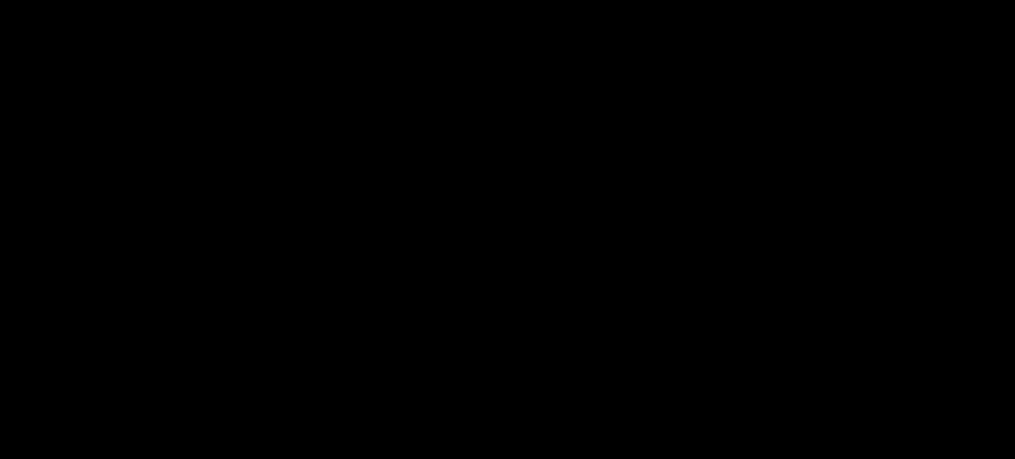
\includegraphics[width=\textwidth]{article1/image.png}
\end{figure}

\title{১ম নিবন্ধের শিরোনাম}
\author{\href{https://github.com/rafisics/ebook-template}{১ম নিবন্ধের লেখক}}
\date{}

% \maketitle                                % Use \maketitle if you want to compile it individually

\section{সেকশন}

\lipsum

% % generates a paragraph of dummy lorem ipsum text
%\blindtext 

% generates multiple paragraphs of dummy lorem ipsum text
% \Blindtext 

% % generates whole document with dummy lorem ipsum text
% \Blinddocument 

\end{document}